\documentclass[11 pt]{article}
\usepackage[all]{xy}
%\documentclass[13pt]{article}
\usepackage{amssymb}
%\usepackage{verbatim}
\usepackage{amsmath}
\usepackage{mathtools}
\usepackage{physics}
\usepackage{setspace}
\usepackage{graphicx}
\usepackage{graphics,graphicx}
\usepackage{pgf,color}
\usepackage{epstopdf}
\usepackage{epsfig,textpos,mathrsfs}
\usepackage{amsthm}
\newtheorem{definition}{Definition}[section]
\usepackage[utf8]{inputenc}
\usepackage[english]{babel}
\usepackage{amsthm}
\usepackage{layout}
%%%%%%%%%%%%%%%%%%%%%%%%%%%%%%%%%%%%%%%%%%%%%%%
\setlength{\textwidth}{6.5in}
\setlength{\textheight}{8.5in}
\setlength{\oddsidemargin}{0pt}
\setlength{\evensidemargin}{0pt}
\setlength{\topmargin}{0pt}
%%%%%%%%%%%%%%%%%%%%%%%%%%%%%%%%%%%%%%%%%%%%%%%
\newtheorem{remark}{Remark}[section]
\newtheorem{theorem}{Theorem}[section]
\newtheorem{lemma}{Lemma}[section]
\newtheorem{proposition}{Proposition}[section]
\newtheorem{corollary}{Corollary}[section]
\newtheorem{example}{Example}[section]
\theoremstyle{definition}
\theoremstyle{remark}
\newcommand{\R}{\mathbb{R}}
\newcommand{\N}{\mathbb{N}}
\newcommand{\h}{\mathcal{H}}
\newcommand{\Z}{\mathbb{Z}}
\newcommand{\B}{\mathcal{B}}
\newcommand{\A}{\mathcal{A}}
\newcommand{\Y}{\mathcal{Y}}
\newcommand{\X}{\mathcal{X}}
\newcommand{\G}{\mathcal{G}}
\newcommand{\T}{\mathbb{T}}
\newcommand{\di}{i} 
\newcommand\norm[1]{\left\lVert#1\right\rVert}
\usepackage{amsmath}
\newcommand{\tens}[1]{
  \mathbin{\mathop{\otimes}\limits_{#1}}}
\linespread{1.1}
\let\conjugatet\overline

\DeclarePairedDelimiterX\set[1]\lbrace\rbrace{\def\given{\;\delimsize\vert\;}#1}


\begin{document}

\begin{center}
\begin{LARGE}
\textbf {Universal quantum computation using the discrete time quantum walk}
\end{LARGE}
\begin{center}
\end{center}
{\begin{Large}
\textbf{MTP REPORT} \\
\end{Large}}
July 2018
%(For enhancement of JRF to SRF)
\end{center}

\vspace{45mm}
\begin{center}
Submitted by


\textbf{Mukesh Bhati}

\bf Entry No. 2013MT60604
\vspace{15mm}

\textit{Supervisor}

\textbf{Dr. N. Shravan Kumar}

\end{center}
\begin{center}
\textbf{{Department of Mathematics\\
Indian Institute of Technology Delhi,\\
New Delhi, INDIA}}
\end{center}
\thispagestyle{empty}
\newpage
\thispagestyle{empty}

\section{Introduction}
The aim of the project is to study and Analysis of different modules used in quantum computation. Then study of discrete time quantum walk and it's application in universal quantum computation. Our aim will be provide a mapping from circuit model to graphical model on which DTQW propagates.     
 \\

\subsection{What is Quantum Computing/Computers ?}
What is quantum computing? It's something that could have been thought up a long time ago. For any physical theory one can ask: what sort of machines will do useful computation? or, what sort of processes will count as useful computational acts? Alan Turing thought about this in 1936 with regard (implicitly) to classical mechanics, and gave the world the paradigm classical computer: the Turing machine. But even in 1936 classical mechanics was known to be false. Work is now under way in seeing what quantum mechanics means for computers and computing.

Quantum computation can be defined as the study of information processing tasks accomplished using quantum mechanical systems. It is a beautiful combination of quantum physics, computer science, and information theory(includes the foundations of both computer science and communications). This is without doubt one of the hottest topics at the current frontiers of
computing and one of the most striking aspects of it is the complete uncertainty about its future.It could rise to meet the expectations of enthusiasts of the field.In such a case, quantum computers will substantially impact our everyday life.


\subsection{Why Quantum Computing/Computers ?}
Quantum Computing/Computers works safer and faster for certain kind of problems than classical computers. Many quantum algorithm are developed that computes faster than classical one. Database search algorithm that can be done using Grover's algorithm having time complexity $O(\sqrt{n})$, gives quadratic speed over classical algorithms.

According to moore's law computer's double every 18th months. Once quantum computers comes into pictures this may end. N-Qubit quantum computer store $2^n$ classical bits. so for large N this may be large number. There are many very good reasons for exploring quantum computing as much as possible.
\begin{itemize}
\item Making use of quantum effects allows one to speed-up certain computations enormously and even enables some things that are impossible for classical computers
\item The process of miniaturization that has made current classical computers so powerful and cheap, has already reached micro-levels where quantum effects occur. Chip-makers tend to go to great lengths to suppress those quantum effects, but instead one might also try to make good use of them.
\end{itemize}

\subsection{Differences between the classical and quantum information processing?}
Classical Information can be read and duplicated. where as quantum computation can not be read in general and can nor be duplicated, but it can be \textbf{teleported}.

The main difference is that quantum information has a special phenomena—called \textbf{Entanglement} which is not available in classical case. This allows that quantum information can be encoded in mutual correlations between remote parts of physical systems.

\section{From Randomized to Quantum Computation}
Comparing Quantum Turing Machine(QTM) to Probabilistic Turing machines(PTM) allows us to find out the difference between basic models of quantum and classical computing. 

\subsection{Probabilistic Turing Machines}
\textbf{probabilistic Turing machine}, having the finite alphabet $\sum$ and a finite set Q of states, is given by a transition function
\begin{center}
$\delta = \sum \times Q \times \sum \times Q \times \{\leftarrow,\downarrow,\rightarrow\} \longrightarrow [0,1]$
\end{center}
meaning that it assign a probability to each possible transition in such a way that the configuration
$c_0$ and all its successor-configurations $c_i$ the local probability condition is satisfied. if $p_i$ is transition probability from $c_0$ to $c_i$ then
\begin{center}
$\sum_{i=1}^{k}p_i = 1$
\end{center}
It is true that if a PTM satisfies all local probability conditions, then it also satisfies
all global probability conditions.

\subsection{Quantum Turing Machines}
Formally, a (one-tape) \textbf{quantum Turing machine}, on a finite set Q of states and the
finite alphabet $\sum$, is given by a transition function
\begin{center}
$\delta = \sum \times Q \times \sum \times Q \times \{\leftarrow,\downarrow,\rightarrow\} \longrightarrow \mathbb{C}_[0,1]$
\end{center}
assigning to each possible transition a probability amplitude in such a way that for each configuration
$c_0$ and all its successor-configurations $c_1, . . ., c_k$ the following local probability condition is satisfied
\begin{center}
$\sum_{i=1}^{k}\left|\alpha_i\right |^2 = 1$
\end{center}
where $\alpha_i$ is transition amplitude from $c_0$ to $c_i$.\newline
It is not true that if a QTM satisfies all local probability conditions, then it also satisfies
all global probability conditions.


\section{Introduction to quantum mechanics}
Quantum mechanics is a mathematical framework or set of rules for the construction of physical theories.
\subsection{ Linear Algebra in Dirac’s Notation}
Dirac’s bra/ket notation is used throughout quantum physics to represent quantum states and their transformations. In Dirac’s notation, a ket such as $\ket{v}$ corresponds to a column vector v, where v is an arbitrary label, refers to a vector representing a state of a quantum system so
\begin{align}
    \ket{v} &= \begin{pmatrix}
           a_{1} \\
           a_{2} \\
           \vdots \\
           a_{m}
         \end{pmatrix}
  \end{align}
In Dirac’s notation, the conjugate transpose of a ket $\ket{v}$ is called a bra and is written $\bra{v}$, so
\begin{align}
\bra{v} &= \begin{pmatrix}
           \conjugatet{a_{1}} & \conjugatet{a_{2}} & \hdots \conjugatet{a_{m}}
         \end{pmatrix}
\end{align}

\subsubsection{Inner Products}

The standard inner product $\braket{a}{b}$ is defined by a function $(.,.)$ from $V \cross V $ to $\mathbb{C}$ which satisfies:\\
1. $(.,.)$ is linear in second argument,
\begin{center}
    $(\ket{a, \sum_{i} C_i \ket{b_i}}) = \sum_{i}C_{i}(\ket{a},\ket{b_i})$
\end{center}
2. $(\ket{a},\ket{b}) = (\ket{b},\ket{a})^*$.\\
3. $(\ket{a},\ket{a}) \geq 0$.\\
4. $(\ket{a},\ket{a}) = 0 \iff \ket{a} =0$

For example, a inner product on $\mathbb{C}$ can be defined by multiplying the conjugate transpose $\bra{a}$= \begin{pmatrix}
    $\conjugatet{a_{1}} & \conjugatet{a_{2}}&\hdots \conjugatet{a_{m}}$
\end{pmatrix} with $\ket{b}$:

\braket{a}{b} = $\bra{a}$ $\ket{b}$ =  
\begin{pmatrix}
    \conjugatet{a_{1}} & \conjugatet{a_{2}} & \hdots \conjugatet{a_{m}} 
\end{pmatrix}
\begin{pmatrix}
           b_{1} \\
           b_{2} \\
           \vdots \\
           b_{m}
         \end{pmatrix}
=\sum_{i=1}^{n}\conjugatet{a_i} b_i.

Dirac’s choice of bra and ket arose as a play on words: an inner product $\braket{a}{b}$ of a bra $\bra{a}$ and a ket $\ket{b}$ is sometimes called a bracket.


A vector $\ket{v}$ can be written as a linear combination of vectors $\ket{s_1}, \ket{s_2}, . . . , \ket{s_n}$ ($\ket{s_i}$ known as basis vectors). If there exist complex numbers $a_i$ such that
\begin{center}
$\ket{v} = a_1\ket{s_1}+a_2\ket{s_2}+$ ··· $+a_n\ket{s_n}$. 
\end{center}
Given a set of vectors S, the subspace of all linear combinations of vectors in S is called the span of S and is denoted span(S). A set of vectors B for which every element of V can be written uniquely as a linear combination of vectors in B is called a basis for V.\newline
In quantum mechanics, bases are usually required to be orthonormal.Two vectors $\ket{v_1}$ and $\ket{v_2}$ are said to be orthogonal if $\braket{v_1}{v_2} = 0$. A set of vectors is orthogonal if all of its members are orthogonal to each other.A set of vectors is said to be orthonormal if all of its elements are of length one and orthogonal to each other: a set of vectors $B = {\ket{\beta_1},\ket{\beta_2}, ... ,\ket{\beta_n}}$ is orthonormal if $\braket{\beta_i}{\beta_j} = \delta_i_j$ for all i,j where
\[ 
\delta_i_j=     \begin{cases} 
                    1 & $if i=j$\\
                    0 & otherwise
                \end{cases}
\]
\textbf{Inner Product Space:} A vector space equipped with an inner product.\\
\textbf{Hilbert Space:} A complete inner product space is known as Hilbert space.\\

In quantum mechanics we are mainly concerned Hilbert spaces, so whenever we say space we mean Hilbert space.\\

\subsubsection{Tensor Products in Hilbert spaces}
Suppose V and W are two Hilbert spaces with bases $B_1 = \{\ket{\alpha_1}, \ket{\alpha_2}, \hdots, \ket{\alpha_n}\}$ and $B_2 = \{\ket{\beta_1}, \ket{\beta_2},
\hdots , \ket{\beta_m}\}$ respectively. Then the tensor product $V \tens{} W$  
i an nm-dimensional vector space with a basis consisting of the nm elements of the form $\ket{\alpha_i} \tens{} \ket{\beta_j}$ where $\tens$ is the tensor product, an abstract binary operator that satisfies the following relations:\\
$(\ket{u} + \ket{v}) \tens{} \ket{w} =  \ket{u} \tens{} \ket{w} + \ket{v} \tens{} \ket{w}$ \\
$\ket{w} \tens{} (\ket{u} + \ket{v}) = \ket{w} \tens{}  \ket{u} + \ket{w} \tens{} \ket{v}$\\
$(a\ket{u}) \tens{} \ket{v} = \ket{u} \tens{} (a\ket{v}) = a(\ket{u} \tens{} \ket{v})$\\
Taking $k = min(n,m)$ , all elements of form $V \tens{} W$ have form\\
$\ket{v_1} \tens{}  \ket{w_1} + \ket{v_2} \tens{}  \ket{w_2} \hdots \ket{v_k} \tens{}  \ket{w_k}$ for some $\ket{v_i} \in V$ and $\ket{w_i} \in W$.
Moreover, all element can be written as
\begin{center}
$v = \sum c_{i,j}(\ket{\alpha_i}\tens{}\ket{\beta_j})$.
\end{center}

\subsubsection{Unitary Operators}
Computation takes place in quantum system through transformation from state space of a closed quantum system to itself. In Quantum system arbitrary transformations do not allowed. The operator used for transformation must respect quantum properties like measurements and super-positions. Also transformation must be linear with state space and should preserve the length of vectors. linearly means
\begin{center}
    $U(a_1\ket{\Phi_1} + a_2\ket{\Phi_2} + \hdots + a_n\ket{\Phi_n}) = a_{1}U\ket{\Phi_1} + \hdots + a_{n}U\ket{\Phi_n}$
\end{center}
 Moreover, first measuring in some basis and then applying a operator $U$ to the outcome should give the same result as first applying the operator $U$ and then measuring in the transformed basis. The above all properties satisfy if operator preserve inner product:
 \begin{center}
     $\bra{\Phi}U^{*}U\ket{\Psi} = \bra{\Phi}\ket{\Psi}$
 \end{center}
 To satisfy above all conditions unitary transformation comes into role. A transformation is called unitary if
\begin{center}
$U^{*}U=\mathbb{I}$
\end{center}
this mean its adjoint $U^{*}$ must be equal to its inverse.
\begin{itemize}
\item U is unitary if and only if the set of columns of its matrix representation are orthonormal.
\item similarly U is unitary if and only if the set of rows of its matrix representation are orthonormal.
\item  The tensor product $U_1 \tens{} U_2$ is a unitary transformation of the space $X_1 \tens{} X_2$ if $U_1$ and $U_2$ are unitary transformations of $X_1$ and $X_2$ respectively.
\end{itemize}



\section{The postulates of Quantum Computing}

\subsection{State Space}
Every isolated physical system has an associated complex vector space with inner product (Hilbert space) called as state space of system. The system's state is described by unit vector, which is known as state vector in system's state space.  

For a given physical system, Quantum mechanics does not tells that what state space is associated with there physical system and what are the state vectors in that state space. we make some assumptions for our propose about state space.\\
1. The most fundamental quantum system concern with qubit.\\
2. State space of qubit is Hilbert space $\mathbb{C}^2$.\\
3. $\ket{0}$ and $\ket{1}$ are orthonormal basis for state space. which we describe by $$\ket{0} = \begin{pmatrix}
           1 \\
           0
\end{pmatrix} \hspace{1cm} \ket{1} = \begin{pmatrix}
           0\\
           1
\end{pmatrix}$$
4. any arbitrary state $\ker{\phi}$ can be written as linear combination of basis states as $$\ket{\phi} = a\ket{0} + \ket{b}$$
where a and b are complex numbers.

\subsection{Evolution}
The time evolution of an isolated or closed quantum system is described by unitary transformation. let at time $t_1$ system is in state $\Phi_1$ and at time $t_2$ the state is $\ket{\Phi_2}$ then $\ket{\Phi_2}$ can be obtain from $\phi_1$ using unitary transformation as follows:
$$\ket{\Phi_2} = U \ket{\Phi_1}$$.
This untary transform preserve its norm. means, if $\Phi$ is a unit vector then $U\phi$ is also an unitary vector. The important unitary operators on a single qubit are:\\
\textbf{Pauli Matrices:} $$I = \begin{pmatrix}
           1 & 0\\
           0 & 1
\end{pmatrix} \hspace{1 cm} X = \begin{pmatrix}
           0 & 1\\
           1 & 0
\end{pmatrix}$$
$$Y = \begin{pmatrix}
           0 & \di\\
           \di & 0
\end{pmatrix} \hspace{1 cm} z = \begin{pmatrix}
           1 & 0\\
           0 & -1
\end{pmatrix}$$

This postulates describe how closed quantum system's quantum states at different times are related to each other. There is more refined version of this postulates whick describe evolution of a quantum system in continuous time using Schrodinger equation. It make use of Hermitian operator.

\subsection{The Qubit}
Let S be a two-dimensional quantum system with two orthonormal states, denoted $\ket{0}$ and $\ket{1}$ that can be considered as forming a standard basis of S. \vspace{5mm} \newline
\textbf{Definition 3.1.1} A \textbf{qubit} is a quantum state 
\begin{center}
 $\ket{\Phi}$ = \alpha$\ket{0}$ + \beta$\ket{1}$
\end{center}
where $\alpha,\beta \in \mathbb{C}$ and $\left|\alpha\right |^2 + \left|\beta\right|^2 $ = 1.\newline
One way we can say that a qubit is a unit vector in two-dimensional inner-product space.for which a particular orthonormal basis, denoted by $\{\ket{0},\ket{1}\}$ has been fixed. This is the fundamental dierence
distinguishing quantum bits from classical ones and is a direct application of the quantum principle of superposition of states.\par
Apart from mathematical defination there are  real physical systems which
may be described in terms of qubits. Possible physical realizations of a qubit include two different polarizations of a photon, the alignment of a nuclear spin in a uniform magnetic field or two electronic levels in an atom.

Since qubit can take any quantum linear superposition of $\ket{0} and \ket{1}$. This means that a large, even infinite, amount of information could potentially be encoded in amplitudes of a single qubit by appropriately choosing $\alpha$ and $\beta$.


\subsection{Quantum Measurements}
Measurements is the amount of information that can be obtain about the state. Theoretically, a qubit can hold an infinite amount of information. However, we cannot extract more information from such a
qubit than we are able to do it from a classical bit. The reason is that we have to measure the qubit in order to determine which state it is in.

Quantum measurement are describe by a collections ${M_n}$ of measurement operator. These operators act on system state space to measure it. Let $\ket{\Phi}$ is the state before measurement then the probability that result m occurs is given by 
$$p(m) = \bra{\Phi|M^{*}M|\ket{\Phi}}$$,
and the state after measurement is given by 
$$ \dfrac{M_m \ket{\Phi}}{\sqrt{\bra{\Phi|M^{*}M|\ket{\Phi}}}}$$
also measurement operators satisfy following conditions,
$$\sum_{m}M_{m}^{*}M_{m} = \mathbb{I}$$.

\textbf{Motivation :} In Postulate 2, we told that quantum system evolve according to unitary evolution. But if an experimenter wants to take measurement with the some equipment then he has to interact with system. It means system is no longer remains closed and hence not subjected to unitary evolution. thus postulate 3 is introduce to tell us about impacts of these measurements on the system.



we measure a qubit 	$\ket{\Phi} = \alpha\ket{0}+\beta\ket{1}$ with respect to the standard basis for quantum computation $\ket{0},\ket{1}$, we get either the result 0 with probability $\left |\alpha\right|^2$ or the result 1 with probability $\left|\beta\right|^2$. The
condition that the probabilities must sum to one corresponds geometrically to the requirement that
the qubit state be normalized to length 1, that is the inner product $\braket{\Phi}$ equals 1.
Thus observing a quantum state induces a probability distribution on the
classical states, given by the squared norms of the amplitudes. measurement outcome is always one of the two basis vectors. For this reason, whenever anyone says “measure a qubit," they must specify with respect to which basis the measurement takes place.
From an
information theory point of view, from a qubit one can obtain by a (projection) measurement
exactly the same amount of (classical) information as a classical bit has, even if it has
infinitely many potential states.

Measurement of a quantum state changes the state. If a state $\ket{\Phi}$ = $\alpha\ket{u} + \beta\ket{u^{\bot}}$ is measured as $\ket{u}$, then the state $\ket{\Phi}$ changes to $\ket{u}$. A second measurement with respect to the same basis will return $\ket{u}$ with probability 1. Because measurement changes the state, one cannot make two measurements on the original state of a qubit.Thus, even though a quantum bit can be in infinitely many different superposition states, it is possible to extract only a single classical bit’s worth of information from a single quantum bit.\newline




\subsection{Superposition}
Let some physical system that can be in N different, mutually exclusive classical states say $\ket{0},\ket{1} .... \ket{N}$. In a classic state mean a state in which the system
can be found if we observe it. but a quantum state can be a superposition
of classical states
\begin{center}
$\ket{\Phi} = \alpha_1\ket{0} + \alpha_2\ket{0}+ ..... +\alpha_N\ket{N} $
\end{center}
Here $\alpha_i$ is a complex number that is called the amplitude of $\ket{i}$ in $\ket{\Phi}$

Mathematically, the states $\ket{1}, ..... \ket{N}$ form an orthonormal basis of an N-dimensional Hilbert space of dimension N, and a
quantum state $\ket{\Phi}$ is a vector in this space.


\subsection{Entanglement}
Entanglement is the correlations between the parts of a system. It can be understand by following two examples:\\
\textbf{e.g. 1.} Suppose you have a 100-page book with print on every page. If you read 10 pages, you'll know 10 percent of the contents. And if you read another 10 pages, you'll learn another 10 percent. But in a highly entangled quantum book, if you read the pages one at a time—or even 10 at a time—you'll learn almost nothing. The information isn't written on the pages. It's stored in the correlations among the pages, so you have to somehow read all of them at once.\\
\textbf{e.g 2.} If Alice and Bob both read this morning's New York Times, they will have perfectly correlated information. And if Charlie comes along and reads the same paper later on, he will be just as strongly correlated with Alice as Alice is with Bob, and Bob will be just as correlated with Charlie as he is with Alice. But if Alice reads her quantum newspaper and Bob reads his, they will learn almost nothing until they get together and share their information. Now, when Charlie comes along, Alice and Bob have already used up all their ability to be entangled, and he's completely left out. Entanglement is monogamous—if Alice and Bob are as entangled as they can be, neither of them can entangle with Charlie at all. So if Alice wants to be entangled with both Bob and Charlie, there's a limit to how entangled she can be with either one. They have to work out some sort of compromise.


\subsection{Quantum Registers}
In classical physics, individual two-dimensional state spaces of n particles combine through the cartesian product to form a vector space of 2n dimensions. However in quantum system Quantum states combine through the tensor product to give a resulting state space of $2^n$ dimensions, for a system of n qubits. Registers is a system comprising multiple qubits which store all information at same time.

For a system of two qubits, each with basis $\{\ket{0},\ket{1}\}$ the resulting state space is the set of normalized vectors in the four dimensional space spanned by basis vectors
$\{\ket{0} \tens{} \ket{0}, \ket{0} \tens{} \ket{1},\ket{1} \tens{} \ket{0},\ket{1} \tens{} \ket{1}\}$ where $\tens{}$ is tensor product. we use compact notation $\{\ket{00},\ket{01},\ket{10},\ket{11}\}$.


\section{Multiple Qubit System}
\subsection{State space of n-qubit system}
suppose $V_i (0 \leq i \leq n-1) $ be the vector spaces, with basis $\{\ket{0}_i,\ket{1}_i\}$, corresponding to a single qubit. The standard basis for the vector space $V_{n-1} \tens{} \hdots \tens{} V_1 \tens{} V_0$ for an n-qubit system consists of the $2^n$ vectors
\begin{center}
$\{\ket{0}_{n-1} \tens{} \hdots \tens{} \ket{0}_1 \tens{} \ket{0}_0,$\\
$\{\ket{0}_{n-1} \tens{} \hdots \tens{} \ket{0}_1 \tens{} \ket{1}_0,$\\
$\{\ket{0}_{n-1} \tens{} \hdots \tens{} \ket{1}_1 \tens{} \ket{0}_0,$\\
$\vdots$\\
$\{\ket{1}_{n-1} \tens{} \hdots \tens{} \ket{1}_1 \tens{} \ket{1}_0,$\\
\end{center}
an even more compact and readable notation uses $\ket{b_{n-1} \hdots b_0}$ to represent $\ket{b_{n-1}} \tens{} \hdots \tens{} \ket{b_0}$.Moreover, the standard basis for an n-qubit system is written $\{\ket{0},\ket{1},\ket{2},\hdots,\ket{{2^n}-1}\}$.

\subsection{Entangled state}
we know a single-qubit state can be specified by a single complex number so any tensor product of n individual single-qubit states can be specified by n complex numbers. but for n-qubit system we need $2^n - 1$ complex numbers to describe states. So n-qubit states cannot be described in terms of the state of n separate single-qubit systems. States that cannot be written as the tensor product of n single-qubit states are called \textbf{entangled states}. Thus the vast majority of quantum states are entangled.  More formally, given a state $\ket{\Phi}$ of some quantum system with associated vector space V and a tensor decomposition of V , $V = V_1 \tens{} \hdots \tens{} V_n$, the state $\ket{\Phi}$ is separable, or unentangled, with respect to that decomposition if it can be written as
\begin{center}
$\ket{\Phi} = \ket{v_1} \tens{} \hdots \ket{v_n}$,
\end{center}
where $\ket{v_i}$ is contained in $V_i$ . Otherwise, $\ket{\Phi}$ is entangled with respect to this decomposition.

\subsection{Measurement in Multiple Qubit System}
\subsubsection{Projection Operator for Measurement}
projective measurement is described by projectors $P_1, . . . , P_m (m ≤ N)$
which sum to identity. These projectors are then pairwise orthogonal, meaning that $P_iP_j = 0$ if
$i \neq j$.
The projector $P_j$ projects on some subspace $V_j$ of the total Hilbert space V , and every state
$\ket{\Phi} \in V$ can be decomposed in a unique way as $\ket{\Phi}= \sum_{j=1}^{m}\ket{\Phi_j}
 $ with $\ket{\Phi_j} = P_j\ket{\Phi} \in V_j$. Because the
projectors are orthogonal, the subspaces $V_j$ are orthogonal as well, as are the states $\ket{\Phi_j}$. When we
apply this measurement to the pure state $\ket{\Phi}$, then we will get outcome j with probability $\norm{\ket{\Phi}}^2 = Tr(P_j\ket{\Phi}\bra{\Phi}) $ and the state will then “collapse” to the new state $\ket{\Phi}/\norm{\ket{\Phi}}=P_j\ket{\Phi}/\norm{P_j\ket{\Phi}}$.

\subsubsection{Hermitian Operator for Measurement}
Hermitian operators can be used for measurements. it uses eigenspace decomposition. Let $O : V \rightarrow V$ be a linear operator. it is called Hermitian if it is equal to its adjoint. And if $O\vec{v}=\lambda\vec{v}$ then $\lambda$ is called eigenvalue and $\vec{v}$ is called eigenvector. set of all eigenvectors correspondence to a $\lambda$ form a eigenspace. from basic linear algebra we know that eigenspaces are orthogonal so every space can be decomposed into direct sum of eigenspaces. means Let V is a N dimensional vector space and $\{\lambda_i\}_{i=1}^{k}$ be k distinct eigenvalues then 
\begin{center}
$V = S_{\lambda_1} \oplus S_{\lambda_2} \oplus \hdots \oplus S_{\lambda_k}$
\end{center}
where $S_{\lambda_i}$ is eigenspace corresponding to $\lambda_i$.\\
let $P_i$ be the projectors onto the subspaces $S_{\lambda_i}$, and let $\lambda_1,\lambda_2,\hdots,\lambda_k$ be any set of distinct real values; then $O = \sum_{i=1}^{k} \lambda_{i}P_i$ is a Hermitian operator with the desired direct sum decomposition.Thus, when describing a measurement, instead of directly specifying the associated subspace decomposition, we can specify a Hermitian operator whose eigenspace decomposition is that decomposition.Any Hermitian operator with the appropriate direct sum decomposition can be used to specify a given measurement; in particular, the values of the λi are irrelevant as long as they are distinct. The λi should be thought of simply as labels for the corresponding subspaces, or equivalently as labels for the measurement outcomes. In quantum physics, these labels are often chosen to represent a shared property, such as the energy, of the eigenstates in the corresponding eigenspace. There are some points in this postulate : 
\begin{itemize}
\item Any quantum measurement can be specified by a Hermitian operator O called an observable.
\item The possible outcomes of measuring a state $\ket{\Phi}$ with an observable O are labeled by the eigenvalues of O. Measurement of state $\ket{\Phi}$ results in the outcome labeled by the eigenvalue $\lambda_i$ of O with probability $\norm{P_{i}\ket{\Phi}}$ where $P_i$ is the projector onto the $\lambda_i$-eigenspace.
\item (Projection) The state after measurement is the normalized projection $P_i\ket{\Phi}/\lVert P_i\ket{\Phi} \rVert$ of $\ket{\Phi}$ onto the eigenspace $S_{\lambda_i}$ . Thus the state after measurement is a unit length eigenvector of O with eigenvalue $\lambda_i$ .
\end{itemize}

\section{Quantum Gates and Quantum circuits}
Quantum circuits is the basic model of quantum computation. A quantum gate is a basic quantum circuit operating on a small number of qubits. In another words any quantum state transformation that acts on only a small number of qubits is called a quantum gate. Sequences of quan- tum gates are called quantum gate arrays or quantum circuits. Unlike many classical logic gates, quantum logic gates are reversible. Quantum logic gates are represented by unitary matrices that can be described by $2^n \times{} 2^n$ sized unitary matrices. The most common quantum gates operate on spaces of one or two qubits. In the following sections we will talk about Some frequently used quantum gates.
\subsection{The Pauli Transformations}
The following are the most commonly used single-qubit transformations:
\subsubsection{Identity Transformation}
\begin{center}
$\mathbb{I} = \ket{0}\bra{0}+\ket{1}\bra{1}$ = 
\begin{bmatrix}
    1  & 0\\
    0  & 1
\end{bmatrix}
\end{center}
\subsubsection{NOT Transformation}
\begin{center}
$\mathbb{X} = \ket{1}\bra{0}+\ket{0}\bra{1}$ = 
\begin{bmatrix}
    0 & 1\\
    1 & 0
\end{bmatrix}
\end{center}
\subsubsection{Phase Transformation}
\begin{center}
$\mathbb{Y} = \ket{0}\bra{0}-\ket{1}\bra{1}$ = 
\begin{bmatrix}
    1  & 0\\
    0  & -1
\end{bmatrix}
\end{center}
\subsubsection{NOT-Phase Transformation}
\begin{center}
$\mathbb{Z} = -\ket{1}\bra{0}+\ket{1}\bra{1}$ = 
\begin{bmatrix}
    0  & 1\\
    -1  & 0
\end{bmatrix}
\end{center}

\subsection{The Hadamard Transformation}
This is used for an even superposition of $\ket{0}$ and $\ket{1}$ from either of the standard basis elements. that is given by
$\mathbb{H} = (1/\sqrt{2})(\ket{0}\bra{0}+\ket{1}\bra{0}+\ket{0}\bra{1}-\ket{1}\bra{1})$
\begin{bmatrix}
    1/\sqrt{2}  & 1/\sqrt{2}\\
    1/\sqrt{2}  & -1/\sqrt{2}
\end{bmatrix}
\\
\\
\\
\\
\\


\begin{center}
\begin{LARGE}
\textbf{II. Quantum Random Walks}
\end{LARGE}
\end{center}

\section{Introduction}
Quantum walks can be considered as a generalized version of the classical random walk. It play an important role in the development of quantum algorithms. Algorithm that are based on quantum walks use a technique called \textbf{amplitude amplification}, which is different from techniques used in algebraic algorithm. In this technique Fourier transform play an important role. The best algorithm to solve element distinctness problem is based on quantum walks. There are two classes of quantum walks, that is, the discrete-time and the continuous-time quantum walks.\\

Before describing the area of quantum walks, we will briefly about classical quantum random walks. we will mainly focus on probability distribution and expected distance from the origin. further we will compare with quantum distance. also we will see that probability of finding the walker away from the origin is greater in the quantum case. This fact is mainly reason the why quantum walks algorithm based on quantum walks can be faster than those based on classical random walks.

\section{Classical Random walk}
\subsection{Random walk on the Line}
The classical random walk in the line is the motion of a particle that lives the set of integers. The particle moves at each time step either one unit to th right with probability p or one unit left with probability 1-p. The directions of different steps are independent of each other and determined by non-biased coin. This classical random walks is known as Bernoulli random walk. Because this process is probabilistic, we cannot know for sure where the particle will be a later time. but we can calculate probability of being it in given state at time t. Following table describe the probabilities of particle in the positions 

\begin{center}
\begin{tabular}{ |c|c|c|c|c|c|c|c|c|c|c|c| } 
 \hline
 t / n   & -5 & -4 & -3 & -2 & -1 & 0 & 1 & 2 & 3 & 4 & 5 \\
 \hline
 0 &  &  &  &  &  & 1 &  &  &  &  &  \\
 \hline
 1 &  &  &  &  & 1/2 &  & 1/2 &  &  &  &  \\
 \hline
 2 &  &  &  & 1/4 &  & 1/2 &  & 1/4 &  &  &  \\
 \hline
 3 &  &  & 1/8 &  & 3/8 &  & 3/8 &  & 1/8 &  &  \\
 \hline
 4 &  & 1/16 &  & 1/4 &  & 3/8 &  & 1/4 &  & 1/16 &  \\
 \hline
 5 & 1/32 &  & 5/32 &  & 5/16 &  & 5/16 &  & 5/32 &  & 1/32 \\
 \hline
\end{tabular}
\end{center}
Figure : Probability of the particle being in the position n at time t, assuming it starts the random walk at the origin. The Probability is zero in empty cells.

\begin{figure}[htp]
\centering
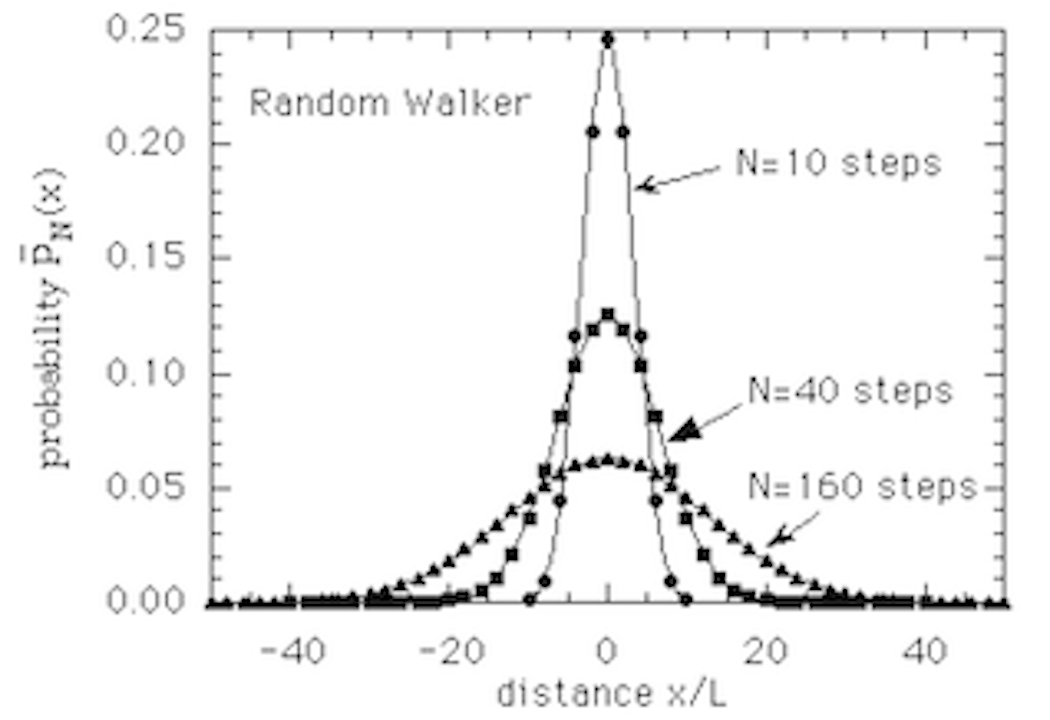
\includegraphics[width=10cm]{Classical_Probability.png}
\caption{Probability distribution of the random walk in a classical one-dimensional lattice for t= 10, t= 40 and t= 160}
\end{figure}
The above figure is for probability distribution of random walk in 1-D. From the curve we can observe that probability is zero for odd values of n when t is even. Another way to interpret the curve of the figure is as the sum $p(t,n) + p(t+1,n) $ i.e. we have two overlapping distributions.\\

There are few observations that can be seen in classical random walk. The first is probability distribution is symmetrical. Second is average position which is zero \\
\begin{center}
    $\mathbb{E}(n) = \sum_{n=-\infty}^{+\infty} np(t,n) = 0$
\end{center}

and standard deviation is 
\begin{center}
    $s.d = \sqrt{\mathbb{E}(n^2) -{\mathbb{E}(n)}^2} = \sqrt{t}$
\end{center}
Thus the variance varies linear with time steps. and also the probability distribution of the random walk can be approximated by the expression
\begin{center}
    $ p(t,n) \simeq \frac{2}{\sqrt{2\pi t}} e^{\frac{-\pi^{2}}{2t}}$
\end{center}


\section{Discrete Time Quantum Walks}
The quantum walk is a quantum generalization of the classical Bernoulli random walk in one dimension with an additional degree of freedom called the chirality. The walk can also be considered as a quantum version of the classical so called correlated random walk. chirality may take value left and right which means direction of the motion of the particle.\\

In a quantum analogue of random walk. it uses 'quantum coin' in place of random walk which has basis states $\ket{+}$ and $\ket{-}$ in dirac notation. Unlike in the classical coin however, the quantum coin can be in
a superposition of states as long as we don't measure it. In other word if $\ket{c}$ is the state after flipping the coin then it can be exist in both simultaneously
\begin{center}
    $\ket{c} = \alpha_{+}\ket{+} + \alpha_{-}\ket{-}$
\end{center}
where $\alpha_{+}$ and $\alpha_{-}$ are amplitudes respectively. If we measure it then it collapse in of the states. hence quantum walk proceeds in absence of measurement or observation. So walker arrives at multiple positions and coin states with various amplitude which constitute a probability wave-function.

Now we generalize the simple quantum walk State of the quantum system is a vector of Hilbert Space and Evolution of the quantum system is Unitary Operator. If we have Unitary operator then there will be no randomness and if we are not totaly isolated then there may be randomness. If we measure the quantum system that will generate the probability distribution.\\

Suppose the Hilbert space is the tensor product of the Hilbert spaces of the components where
\hspace{3cm} $H_{p} = $Position Hilbert space\\
\hspace{3cm} $H_{c} = $Coin Hilbert space\\
\hspace{3cm}So Hilbert space of the system \\
\begin{center}
    $H = H_{p} \tens{} H_{c}$
\end{center}
where computational basis of $H_{c}$ is $= \{\ket{+},\ket{-}\}$ and $H_{p}$ is $= \{\ket{x} : x\in \mathbb{Z} \}$

In quantum case, the walker's position n should be a vector in Hilbert space $H_{p}$. Evolution of walk depends on quantum coin. The complete state of walker can be describe as a super positions of all given states
\begin{center}
    $\ket{\Phi} = \sum_{x} \alpha_{x,-}\ket{x,-} + \alpha_{x,+}\ket{x,+}$
\end{center}
\\
For the coin state transfer it use coin operator which is unitary operator and then unitary conditional translation operator or shift operator which shift the state corresponding the coin state. So in single step of a quantum walk involves a simultaneously application of coin operator followed by translation operator across all the states. And also making measurement at every step would collapse it into one of the step with some probability. Hence quantum walk proceeds in absence of measurement or observation\\
\textbf{Shift Operator}\\
The shift from $\ket{x}$ to $\ket{x+1}$ or $\ket{x-1}$ must be described by a unitary operator, called the shift operator S. It should operate as follow,
\begin{center}
    $ S \ket{+}\ket{x} = \ket{+} \ket{x+1}$
    $ S^* \ket{-}\ket{x} = \ket{-} \ket{x-1}$
\end{center}\\
So for above transformation we can define in following way
\begin{center}
    $S = \sum_{x \in \mathbb{Z}} \ket{x+1}\bra{x}$ and 
    $S^* = \sum_{x \in \mathbb{Z}} \ket{x-1}\bra{x}$
\end{center}
\textbf{Quantum walk Unitary Operator}
\begin{center}
    $U = S ( H \tens{} I)$
\end{center}
where H is Hadamard coin, the most used coin in 1-D walk.\\
\\
\textbf{Recursive formula based method:}\\
The generic state of the quantum walk can be written as a linear combination of the computational basis as
\begin{center}
    $\ket{\Phi_n(x)} = \sum_{-\infty}^{\infty} (A_{x}(n)\ket{-} +(B_{x}(n)\ket{+}) \ket{x}$
\end{center}
where 
\begin{center}
    $ \sum_{-\infty}^{\infty} \abs{(A_{x}(n)}^2 + \abs{(B_{x}(n)}^2 = 1$
\end{center}
When applying $H \tens{} I $ followed by the shift operator, we can obtain recursive formulas involving the coefficients A and B, which are given by
\begin{center}
    $A_{x}(n+1) = \dfrac{A_{x-1}(n) + B_{x-1}(n)}{\sqrt{2}}$\\
    $B_{x}(n+1) = \dfrac{A_{x+1}(n) - B_{x+1}(n)}{\sqrt{2}}$
\end{center}
where initial condition is given by
\[ 
A_{x}(n)=     \begin{cases} 
                    1 & $if x=0$\\
                    0 & otherwise
                \end{cases}
\]
and $B_{x}(n)=0$.

Then we can easily find the probability distribution
$$ P(n,x) = \abs{(A_{x}(n)}^2 + \abs{(B_{x}(n)}^2 $$

\subsection{More on Quantum walk}
Here we will discuss the characteristic function of quantum random walk and dependence of m-th moment, symmentry of the distribution on the matrix U and the initial qubit state \Phi.
\subsubsection{Two State Case}
The quantum walk can be determined a 2 \cross 2 unitary matrix U that we can define in following way
\begin{center}
     U = \begin{bmatrix}
                a & b\\
                c & d
         \end{bmatrix}
\end{center}
where a,b,c,d $\in \mathbb{C}$. Quantum walk have additional degree of freedom called chirality which can values left and right. Moreover U acts on two chirality states $\ket{L}$ and $\ket{R}$:
$$ \ket{L} \rightarrow a\ket{L} + c\ket{R},
   \ket{R} \rightarrow b\ket{L} + d\ket{R}$$

Let $X_n$ be the quantum random walk at time n starting from initial qubit state $\Phi \in \Phi$. where $\Phi$ is set of initial qubit states as follows:
$$\Phi = \set[\bigg]{\Phi = \begin{bmatrix}
                    \alpha\\
                    \beta
                \end{bmatrix}
                \in \mathbb{C} : \abs{\alpha}^2 + \abs{\beta}^2 =1}
$$
we define two matrix P and Q :
$$P = \begin{bmatrix}
        a & b\\
        0 & 0
\end{bmatrix}, Q = \begin{bmatrix}
        0 & 0\\
        c & d
\end{bmatrix}$$
Remark that $$ U = P + Q$$.
We will see that quantum walk behaves differently from classical random walks. Probability distribution of classical walk is bionomial disrtibution where as in quantum walk it has a complicated, oscillatory form. Also symmetry of distribution depends on initial qubit states.\\

Let $\Phi_n(x)$ be the two dimensional vector of amplitudes of the particle being at site x and at time n then state is define as :
$$\Phi_n(x) = \begin{bmatrix}
                \Phi_{n}^L(x)\\
                \Phi_{n}^R(x)
\end{bmatrix}   = \Phi_{n}^L(x)\ket{L} + \Phi_{n}^R(x)\ket{R} \in \mathbb{C}^2$$
and after N steps  $$ \Phi_n = \begin{bmatrix}
        \Phi_n(-N),\Phi_n(-(N-1) \hdots \Phi_n(N)
\end{bmatrix}$$
also we introduce unitary matrix $\overline{U}_N$ $(2N+1) \cross (2N+1)$  as
$$ \overline{U}_N = \begin{bmatrix}
                0 & P & 0 & \hdots & \hdots & 0 & Q\\
                Q & 0 & P & 0 & \hdots & \hdots & 0\\
                0 & Q & 0 & P & 0 & \hdots & 0\\
                \vdots & \vdots & \vdots & \vdots & \vdots & \hdots & \vdots\\
                0 & \hdots & 0 & Q & 0 & P & 0\\
                0 & \hdots & \hdots & 0 & Q & 0 & P\\
                P & 0 & \hdots & \hdots & 0 & Q & 0
\end{bmatrix}$$
Here P represent the left chirality and Q represent right chirality.
\newpage
The following equation defines the time evolution of the quantum walk:
$$  \Phi_{n+1}(x) = (\overline{U}_N\Phi_n)_x = P\Phi_n(x+1) + Q\Phi_n(x-1)$$
where $-N \leq x \leq N$ and $1 \leq n \leq N.$

Let $\ket{x} \in H_p$ be the position states of the quantum walk. A unitary shift operator is defined in following way  
\begin{center}
    $S = \sum_{x \in \mathbb{Z}} \ket{x+1}\bra{x}$ and 
    $S^* = \sum_{x \in \mathbb{Z}} \ket{x-1}\bra{x}$
\end{center}
If $\Hat{P} = \ket{L}\bra{L}$ and $\Hat{Q}= \ket{R}\bra{R}$ are two projection operator on coin state then Unitary operator on one step walk is given by:
$$  U = ( S \tens{} \Hat{Q} + S^* \tens{} \Hat{P})(I \tens{} H)$$
So after n step the state is 
$$\Phi_n = \overline{U}^n\Phi_0$$
\\
\textbf{Possible path trajectory}\\
for fixed l and m with l+ m = n and -l + m = x we consider $\Xi_n(l,m)$ the sum of all possible paths in the trajectory is given by :
$$ \Xi_n(l,m) = \sum_{l_j,m_j} P^{l_1}Q^{m_1} \hdots P^{l_n}Q^{m_n}  $$
satisfying $l_1 + l_2 + \hdots + l_n=l, m_1 + m_2+ \hdots +m_n = m$ and $l_j + m_j = 1$.
we also note that
$$ \Phi_n(x) = \Xi_n(l,m) \varphi$$ where $\varphi$ is initial state.\\
\textbf{Example}: for $P(X_4 =-2)$ the possible path is given by
$$  \Xi_n(3,1) = QP^3 + PQP^2 + P^2QP + P^3Q$$
\\
We introduce two matrices R and S as
$$  R= \begin{bmatrix}
        c&d\\
        0&0
\end{bmatrix}, S=\begin{bmatrix}
    0&0\\
    a&b
\end{bmatrix}$$
we also note that
\begin{center}
\begin{tabular}{ c | c  c  c  c  }
   & P & Q & R & S\\
   \hline
  P & aP & bR & aR & bP\\
  Q & cS & dQ & cQ & dS\\
  R & cP & dR & cR & dP\\
  S & aS & bQ & aQ & bS
\end{tabular}
\end{center}
Using this above table we get expression of $\Xi_n(l,m)$ in following form $$\Xi_n(l,m) = p_n(l,m)P +q_n(l,m)Q +r_n(l,m)R + s_n(l,m)S $$
in our example we get by solving
    $$\Xi_4(3,1) = 2abcP + a^2bR + a^2cS.$$
\\
\textbf{Lemma 1.1.} (i) for $l \wedge m(= min{l,m}) \geq 1$ , 
$$\Xi_n(l,m) = a^l\overline{a}^m \triangle^m \sum_{\gamma=1}^{l\wedge m} \bigg(-\frac{\abs{b}^2}{\abs{a}^2}\bigg)^{\gamma} \binom{l-1}{\gamma-1}\binom{m-1}{\gamma-1} \cross \bigg[\frac{l-\gamma}{a\gamma}P + \frac{m-\gamma}{\triangle\overline{a}\gamma}Q + \frac{1}{\triangle\overline{b}}R + \frac{1}{b}S}\bigg]  $$
\\
(ii) for l(=n), m=0
$$\Xi_n(l,0) = a^n-1P$$
\\
(iii) for l=0, m(=n)
$$\Xi_n(0,m) = \triangle^n-1 \overline{a}^{n-1}Q$$
\\
by using lemma 1 we can derive the distribution of $X_n$ that is given in lemma 2.
\\
\textbf{lemma 1.2.} for k = 1,2, $\hdots$ [n/2] we have\\

$ P(X_n=n-2k) 

= \abs{a}^{2(n-1)}\sum_{\gamma=1}^{k}\sum_{\delta=1}^{k}
                 \bigg(-\frac{\abs{b}^2}{\abs{a}^2}\bigg)^{\gamma+\delta}
                 \binom{k-1}{\gamma-1}\binom{k-1}{\delta-1}\binom{n-k-1}{\gamma-1}\binom{n-k-1}{\delta-1}\\
                 \hspace{3cm}\cross\bigg(\frac{1}{\gamma\delta}\bigg)\bigg[{k^2\abs{a}^2 + (n-k)^2\abs{b}^2 -(\gamma+\delta)(n-k)}\abs{\alpha}^2 +
                 k^2\abs{b}^2 + (n-k)^2\abs{a}^2 -(\gamma+\delta)(k)}\abs{\beta}^2+\frac{1}{\abs{b}^2}\\
                 \big[{(n-k)\gamma-k\delta +n(2k-n)\abs{b^2}}a\alpha\overline{b\beta} + {-k\gamma + (n-k)\delta + n(2k-n)\abs{b}^2}\overline{a\alpha}b\beta + \gamma\delta \big]\bigg] $\\
                 
\textbf{and}\\ 
                 
$ P(X_n=-(n-2k)) 

= \abs{a}^{2(n-1)}\sum_{\gamma=1}^{k}\sum_{\delta=1}^{k}
                 \bigg(-\frac{\abs{b}^2}{\abs{a}^2}\bigg)^{\gamma+\delta}
                 \binom{k-1}{\gamma-1}\binom{k-1}{\delta-1}\binom{n-k-1}{\gamma-1}\binom{n-k-1}{\delta-1}\\
                 \hspace{3cm}\cross\bigg(\frac{1}{\gamma\delta}\bigg)\bigg[{k^2\abs{b}^2 + (n-k)^2\abs{a}^2 -(\gamma+\delta)(k)}\abs{\alpha}^2 +
                 k^2\abs{a}^2 + (n-k)^2\abs{b}^2 -(\gamma+\delta)(n-k)}\abs{\beta}^2+\frac{1}{\abs{b}^2}\\
                 \big[{(k)\gamma-(n-k)\delta -n(2k-n)\abs{b^2}}a\alpha\overline{b\beta} + {-(n-k)\gamma + (k)\delta - n(2k-n)\abs{b}^2}\overline{a\alpha}b\beta + \gamma\delta \big]\bigg] $

\begin{figure}
    \centering
    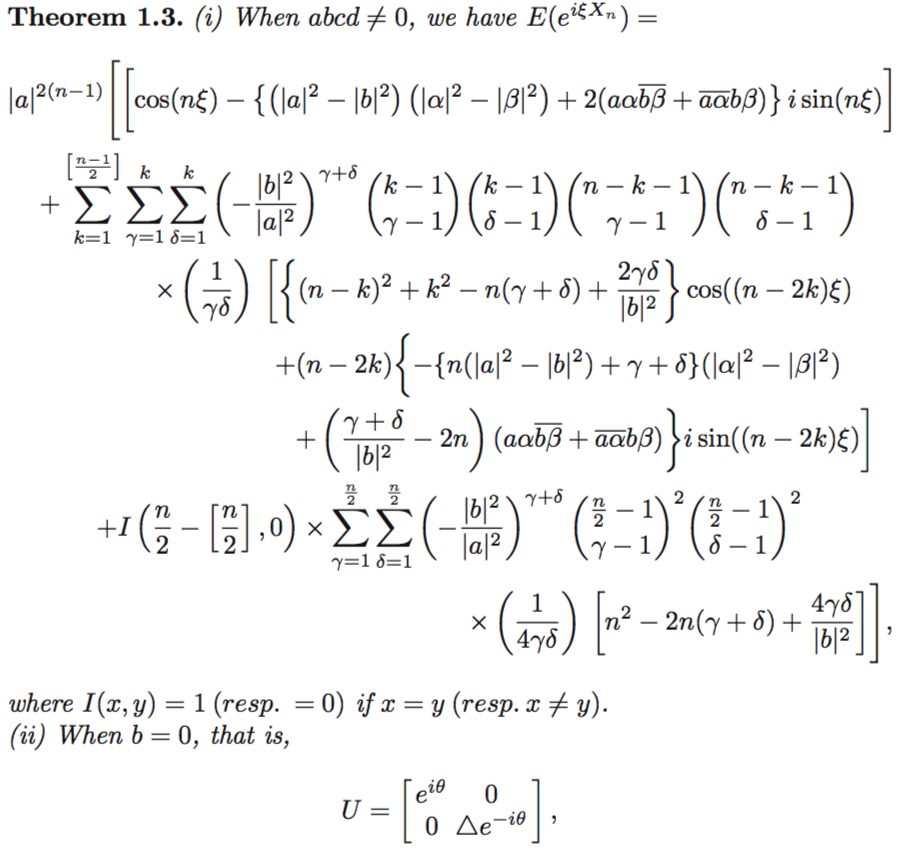
\includegraphics[width=15cm]{Thm1.png}
    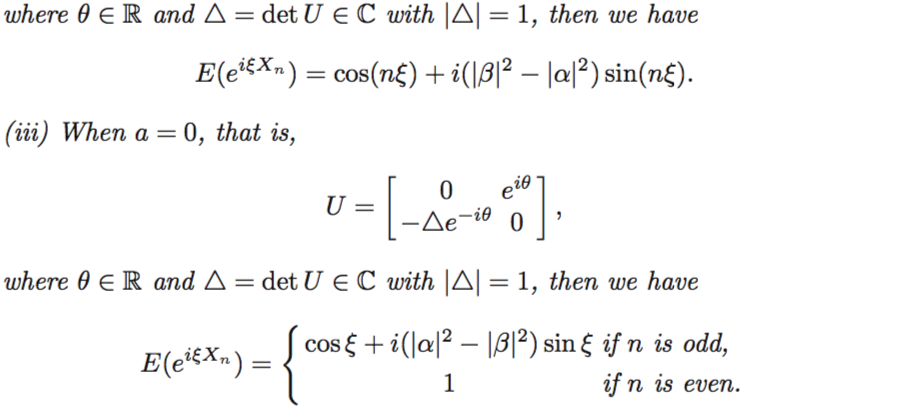
\includegraphics[width=15cm]{Thm1_1.png}
\end{figure}
\\
by using above theorem we get m-th moment of $X_n$  which can be express in following way
\begin{figure}
    \centering
    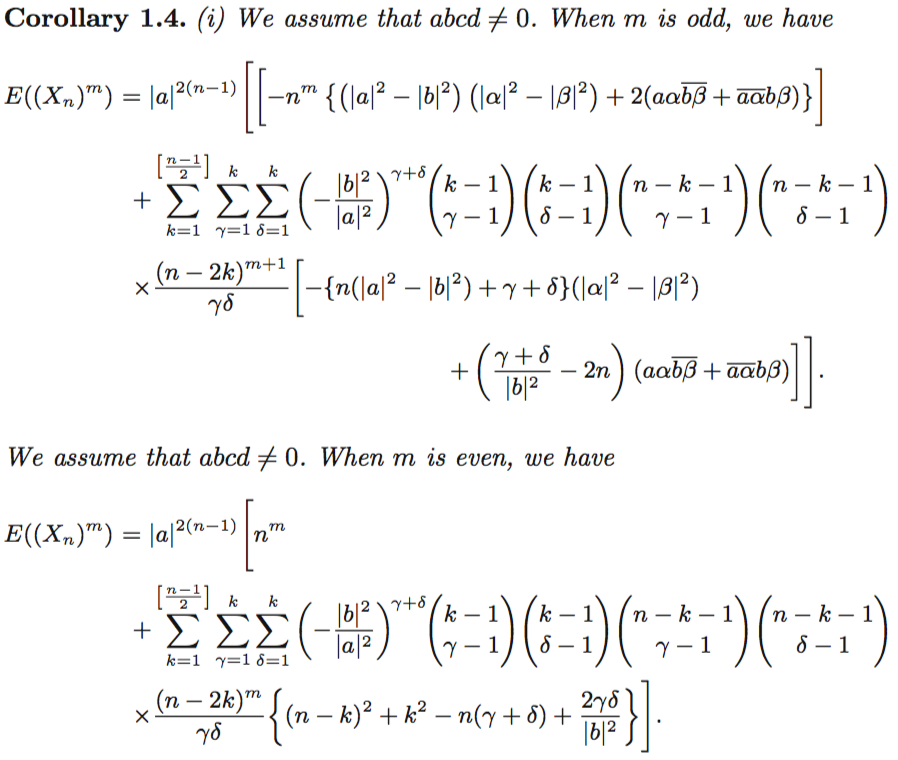
\includegraphics[width=15cm]{Thm2.png}
    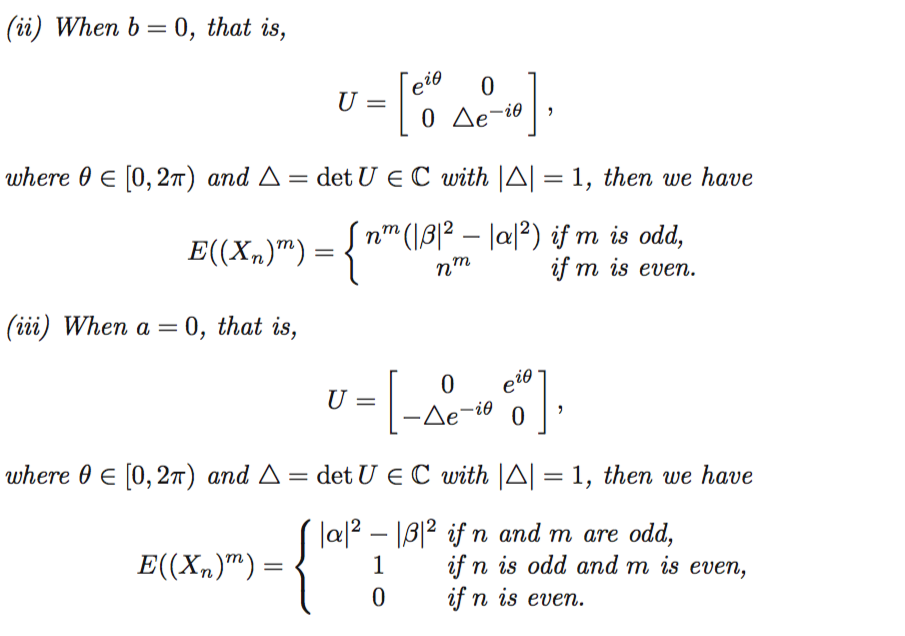
\includegraphics[width = 15cm]{Thm2_1.png}
\end{figure}
we can clearly see that if m is even, the m-th moment is independent of initial qubit state $\Phi$ whereas m is odd, its depend on initial state.
\\
\\
\textbf{Fourier Analysis}\\
\\
Fourier transformation of state is the relation
$$
\hat{\Phi}_{n}^{j}(k) = \sum_{x \in Z}e^{-ikx}\Phi_{n}^{j}(x)$$\\
$$
\Phi_{n}^{j}(x) = \int_{-\pi}^{\pi} \frac{dk}{2\pi}e^{ikx}\hat{\Phi}_{n}^{j}(x)
$$
In wave number space(k-space) of Fourier transformation $k \in [-\pi,\pi]$ as $$ \hat{\Phi}_{n+1}(k) = U(k)\hat{\Phi}_n(k)$$ , $n=0,1,2, \hdots$.
where U(k) is given by
$$
U(k) = \begin{bmatrix}
    e^ik & 0\\
    0 & e^{-ik}
\end{bmatrix}U
$$
and The state after n step can be given as 
$$
\hat{\Phi}_{n+1}(k) = U(k)^{n}\hat{\Phi}_n(k)
$$
\\
\\
\textbf{Weak Limit Theorem}\\
\\
\textbf{Theorem 1.5} If $n \rightarrow \infty$ , then 
                        $$ \frac{X_n}{n} \implies Z$$,
where Z has a density function\\

 $f(x) = f(x ; \Phi = [\alpha, \beta]^T)
 = \dfrac{\sqrt{1-\abs{a}^2}}{\pi(1-x^2)\sqrt{\abs{a}^2 - x^2}}
 \bigg \{
 1-\bigg(\abs{\alpha}^2 -\abs{\beta}^2 +
 \dfrac{a\alpha\overline{b\beta} + \overline{a\alpha}b\beta}{\abs{a}^2}\bigg)x\bigg \}$, \\
 \\
 for $ x \in (-\abs{a},\abs{a}) and f(x) =  for \abs{x} \geq \abs{a}$ with\\
 $$E(Z) = -\bigg(\abs{\alpha}^2 -\abs{\beta}^2 + \dfrac{a\alpha\overline{b\beta} + \overline{a\alpha}b\beta}{\abs{a}^2}\bigg) \cross (1-\sqrt{1-\abs{a}^2})$$
 \hspace{3.25cm}$E(Z^2) = 1 - \sqrt{1-\abs{a}^2}$
\\


\section{References}
\begin{itemize}
\item A. Kitaev, A. Shen, and M. Vyalyi. Classical and Quantum Computation, volume 47 of Graduate Studies in Mathematics. American Mathematical Society, 2002.
\item Rieffel E.G. and Wolfgang H.P. quantum computing a gentle introduction.
\item M.A. Nielsen and I.L. Chuang Quantum computation and quantum information, Cambridge University Press, 2000.
\item Jozef Grusa Introduction to Quantum Computing.
\item Norio Konno, Philiphe Biane, Quantum Potential Theory, Lecture Notes in Mathematics 2008
\item J. Kempw. Quantum random walk:an introductory overview. Contemp. Phy. 2003
\item R. Portugal, Quantum walks and search algorithm Springer, 2013
\end{itemize}

\end{document}


